%Dạng 1
\setcounter{ex}{0}
\section{Nhận dạng đồ thị hàm số}
\subsection{Kiến thức cần nhớ}
\begin{khung}
\subsubsection{ Hàm số bậc 3: $y=ax^3+bx^2+cx+d$ \, $(a\neq 0)$}
\renewcommand{\arraystretch}{1} %Thay đổi độ rộng các dòng
\begin{center}
	\begin{tabular}{|m{4.3cm}|m{5.5cm}|m{5.5cm}|}
	\hline
	\textbf{Trường hợp}	& $$a>0$$	& $$a<0$$\\
	\hline
	{$y'=0$ có 2 nghiệm phân biệt ($b^2-3ac>0$)}	& 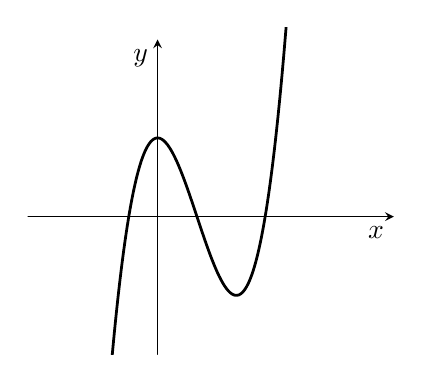
\begin{tikzpicture}[line cap=round,line join=round,>=stealth,x=.5cm,y=.5cm]
		\clip(-3.3,-3.5) rectangle (6.2,4.8);
		\draw[->] (-3.3,0)--(6,0) node[below left]{$x$};
		\draw[->] (0,-3.5)--(0,4.5) node[below left]{$y$};
		\draw[line width=1pt,color=black,smooth,samples=200,domain=-3.3:6] plot(\x,{(\x)^(3.0)-3.0*(\x)^(2.0)+2.0});
	\end{tikzpicture} 	& 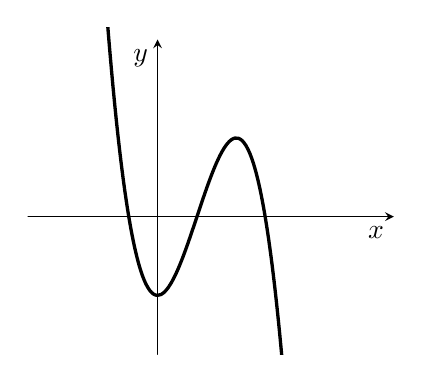
\begin{tikzpicture}[line cap=round,line join=round,>=stealth,x=.5cm,y=.5cm]
		\clip(-3.3,-3.5) rectangle (6.2,4.8);
		\draw[->] (-3.3,0)--(6,0) node[below left]{$x$};
		\draw[->] (0,-3.5)--(0,4.5) node[below left]{$y$};
		\draw[line width=1.2pt,color=black,smooth,samples=100,domain=-3.3:6] plot(\x,{-1*(\x)^(3.0)+3.0*(\x)^(2.0)-2.0});
	\end{tikzpicture}\\
	\hline
	%-------------------
	$y'=0$ có nghiệm kép hoặc vô nghiệm ($b^2-3ac\leq 0$)	& \begin{tikzpicture}[line cap=round,line join=round,>=stealth,x=.5cm,y=.5cm]
		\clip(-3.3,-3.5) rectangle (6.2,4.8);
		\draw[->] (-3.3,0)--(6,0) node[below left]{$x$};
		\draw[->] (0,-3.5)--(0,4.5) node[below left]{$y$};
		\draw[line width=1.2pt,color=black,smooth,samples=100,domain=-3.3:6] plot(\x,{(\x)^(3.0)+2.0*(\x)^(2.0)+1.5*(\x)+0.5});
	\end{tikzpicture}	& \begin{tikzpicture}[line cap=round,line join=round,>=stealth,x=.5cm,y=.5cm]
		\clip(-3.3,-3.5) rectangle (6.2,4.8);
		\draw[->] (-3.3,0)--(6,0) node[below left]{$x$};
		\draw[->] (0,-3.5)--(0,4.5) node[below left]{$y$};
		\draw[line width=1.2pt,color=black,smooth,samples=100,domain=-3.3:6] plot(\x,{0-(\x)^(3.0)-2.0*(\x)^(2.0)-1.5*(\x)+0.5});
	\end{tikzpicture}\\
	
	\hline
\end{tabular} 
\end{center}

\subsubsection{ Hàm số trùng phương $y=ax^4+bx^2+c$ \, $(a\neq 0)$}

\begin{center}
	\begin{tabular}{|m{4.3cm}|m{5.5cm}|m{5.5cm}|}
	\hline 
	\textbf{Trường hợp} & $$a>0$$ & $$a<0$$ \\ 
	\hline 
	Phương trình $y'=0$ có $3$ nghiệm phân biệt ($a.b<0$) & 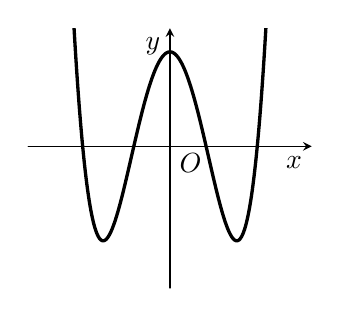
\begin{tikzpicture}[scale=0.6,line cap=round,line join=round,>=stealth]
		\draw[->,color=black] (-3,0) -- (3,0) node[below left]{$x$};
		\draw[->,color=black] (0,-3) -- (0.,2.5)  node[below left]{$y$};
		\draw[color=black] (0pt,-10pt) node[right] {$O$};
		\clip(-3,-3) rectangle (3,2.5);
		\draw[line width=1.2pt,color=black,smooth,samples=200,domain=-3:3] plot(\x,{(\x)^(4.0)-4.0*(\x)^(2.0)+2.0});
	\end{tikzpicture} & 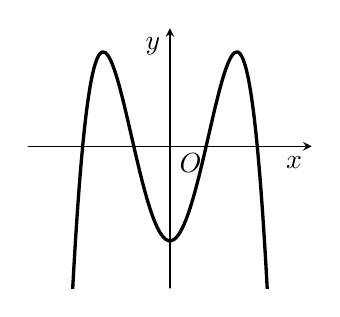
\begin{tikzpicture}[scale=0.6,line cap=round,line join=round,>=stealth]
		\draw[->,color=black] (-3,0) -- (3,0) node[below left]{$x$};
		\draw[->,color=black] (0,-3) -- (0.,2.5) node[below left]{$y$};
		\draw[color=black] (0pt,-10pt) node[right] {$O$};
		\clip(-3,-3) rectangle (3,2.5);
		\draw[line width=1.2pt,color=black,smooth,samples=100,domain=-3.0:3.0] plot(\x,{0-(\x)^(4.0)+4.0*(\x)^(2.0)-2.0});
	\end{tikzpicture} \\ 
	\hline 
	Phương trình $y'=0$ có $1$ nghiệm ($a.b\geq 0$) &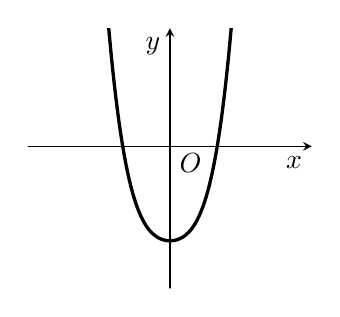
\begin{tikzpicture}[scale=0.6,line cap=round,line join=round,>=stealth]
		\draw[->,color=black] (-3,0) -- (3,0) node[below left]{$x$};
		\draw[->,color=black] (0,-3) -- (0.,2.5) node[below left]{$y$};
		\draw[color=black] (0pt,-10pt) node[right] {$O$};
		\clip(-3,-3) rectangle (3,2.5);
		\draw[line width=1.2pt,color=black,smooth,samples=100,domain=-3.0:3.0] plot(\x,{(\x)^(4.0)+(\x)^(2.0)-2.0});
	\end{tikzpicture} & 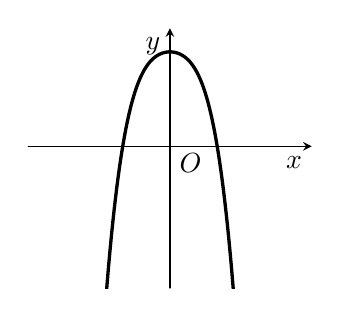
\begin{tikzpicture}[scale=0.6,line cap=round,line join=round,>=stealth]
		\draw[->,color=black] (-3,0) -- (3,0) node[below left]{$x$};
		\draw[->,color=black] (0,-3) -- (0.,2.5) node[below left]{$y$};
		\draw[color=black] (0pt,-10pt) node[right] {$O$};
		\clip(-3,-3) rectangle (3,2.5);
		\draw[line width=1.2pt,color=black,smooth,samples=100,domain=-3.0:3.0] plot(\x,{0-(\x)^(4.0)-(\x)^(2.0)+2.0});
	\end{tikzpicture} \\ 
	\hline 
\end{tabular} 

\end{center}

\subsubsection{ Hàm số nhất biến $y=\dfrac{ax+b}{cx+d},\left(ab-bc\neq 0\right)$}
\begin{center}
	\begin{tabular}{|m{6cm}|m{6cm}|}
		\hline 
		\begin{center}
			Khi $ad-bc>0$
		\end{center} & \begin{center}
			Khi $ad-bc<0$
		\end{center} \\ 
		\hline 
		\begin{tikzpicture}[scale=0.7,>=stealth, font=\footnotesize, line join=round, line cap=round]
			\def\a{1} \def\b{1} \def\c{-1} \def\d{1}
			\draw[->] (-3,0)--(4.2,0) node [below]{$x$};
			\draw[->] (0,-3.7)--(0,2.7) node [below left]{$y$};
			\node at (0,0) [below left=-1pt]{$O$};
			\clip (-2.9,-3.6) rectangle (4.2,2.6);
			\draw[smooth,samples=300,domain=-3:(-\d/\c-0.1)] plot(\x,{(\a*(\x)+\b)/(\c*(\x)+\d)});
			\draw[smooth,samples=300,domain=(-\d/\c+0.1:4.2)] plot(\x,{(\a*(\x)+\b)/(\c*(\x)+\d)});
			\draw[dashed] (-\d/\c,-3.7)--(-\d/\c,2.7);
			\draw[dashed] (-3,\a/\c)--(4.2,\a/\c);
		\end{tikzpicture} & 	\begin{tikzpicture}[scale=0.7,>=stealth, font=\footnotesize, line join=round, line cap=round]
			\def\a{1} \def\b{2} \def\c{2} \def\d{-1}
			\draw[->] (-3,0)--(4.2,0) node [below]{$x$};
			\draw[->] (0,-3.7)--(0,2.7) node [below left]{$y$};
			\node at (0,0) [below left=-1pt]{$O$};
			\clip (-2.9,-3.6) rectangle (4.2,2.6);
			\draw[smooth,samples=300,domain=-3:(-\d/\c-0.1)] plot(\x,{(\a*(\x)+\b)/(\c*(\x)+\d)});
			\draw[smooth,samples=300,domain=(-\d/\c+0.1:4.2)] plot(\x,{(\a*(\x)+\b)/(\c*(\x)+\d)});
			\draw[dashed] (-\d/\c,-3.7)--(-\d/\c,2.7);
			\draw[dashed] (-3,\a/\c)--(4.2,\a/\c);
			%\foreach \x in {-2,-1,1}
			%\draw (\x,0.05)node[below]{$\x$}--(\x,-0.05);
			%\foreach \y in {-1,1,2}
			%\draw (-0.05,\y)node[right]{$\y$}--(0.05,\y);
		\end{tikzpicture}\\ 
		\hline 
	\end{tabular} 
\end{center}
\end{khung}
\subsection{Bài tập mẫu}
\Opensolutionfile{ans}[ans/ANS-DANG-9]
\begin{khung}
%Cau 9
\begin{vd}[De Tham khao BGD 2023]%[2D1Y5-1]
	\immini{Đồ thị của hàm số nào dưới đây có dạng như đường cong trong hình bên
		\choice
		{$y=x^4-3x^2+2$}
		{\True $y=\dfrac{x-3}{x-1}$}
		{$y=x^2-4x+1$}
		{$y=x^3-3x-5$}
	}{\begin{tikzpicture}[>=stealth,font=\scriptsize,scale=.45,
			declare function={hsf(\x)=(\x-3)/(\x-1);}]
			\draw[->] (-3.5,0)--(0,0)node[below left]{$O$}--(5.5,0) node[below]{$x$};
			\draw[->] (0,-3.5)--(0,5.5) node [left]{$y$};
			\draw[blue,smooth,samples=100] plot[domain=1.45:5.2](\x,{hsf(\x)}) plot[domain=-3.2:.55](\x,{hsf(\x)});
			\draw(1,5.25)--(1,-3.25) (-3.2,1)--(5.2,1);
	\end{tikzpicture}}
	\loigiai{
		Đồ thị của hàm số $y=\dfrac{x-3}{x-1}$ có dạng như đường cong trong hình.
	}
\end{vd}
\end{khung}

\subsection{Bài tập tương tự và phát triển}

\begin{ex}%[Đỗ Đường Hiếu, ĐMH-2023]%[2D1Y5-1]
Đồ thị hàm số $y=-x^4+2x^2$ là hình nào sau đây?
\choice
{\begin{tikzpicture}[scale=0.8, font=\footnotesize,line join=round, line cap=round,>=stealth]
			\draw[->] (-2,0)--(0,0)node[below left]{$O$}--(2,0) node[below]{$x$};
			\draw[->] (0,-3)--(0,1) node [left]{$y$};
			\begin{scope}
				\clip (-2,-3) rectangle (2,1);
				\draw[blue,smooth,samples=100] plot[domain=-2:2](\x,{-(\x)^2-1});
			\end{scope}
			\fill[black] (0,0) circle(1pt);
\end{tikzpicture}}
{\True 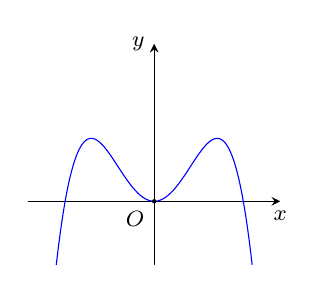
\begin{tikzpicture}[scale=0.8, font=\footnotesize,line join=round, line cap=round,>=stealth]
		\draw[->] (-2,0)--(0,0)node[below left]{$O$}--(2,0) node[below]{$x$};
		\draw[->] (0,-1)--(0,2.5) node [left]{$y$};
		\begin{scope}
			\clip (-2,-1) rectangle (2,2);
			\draw[blue,smooth,samples=100] plot[domain=-2:2](\x,{-(\x)^4+2*(\x)^2});
		\end{scope}
		\fill[black] (0,0) circle(1pt);
\end{tikzpicture}}
{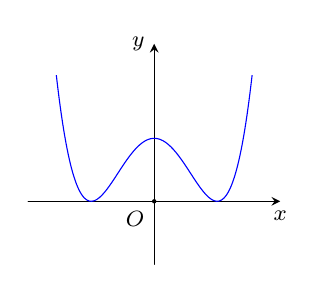
\begin{tikzpicture}[scale=0.8, font=\footnotesize,line join=round, line cap=round,>=stealth]
		\draw[->] (-2,0)--(0,0)node[below left]{$O$}--(2,0) node[below]{$x$};
		\draw[->] (0,-1)--(0,2.5) node [left]{$y$};
		\begin{scope}
			\clip (-2,-1) rectangle (2,2);
			\draw[blue,smooth,samples=100] plot[domain=-2:2](\x,{(\x)^4-2*(\x)^2+1});
		\end{scope}
		\fill[black] (0,0) circle(1pt);
\end{tikzpicture}}
{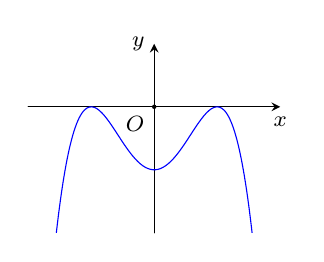
\begin{tikzpicture}[scale=0.8, font=\footnotesize,line join=round, line cap=round,>=stealth]
		\draw[->] (-2,0)--(0,0)node[below left]{$O$}--(2,0) node[below]{$x$};
		\draw[->] (0,-2)--(0,1) node [left]{$y$};
		\begin{scope}
			\clip (-2,-2) rectangle (2,1);
			\draw[blue,smooth,samples=100] plot[domain=-2:2](\x,{-(\x)^4+2*(\x)^2-1});
		\end{scope}
		\fill[black] (0,0) circle(1pt);
\end{tikzpicture}}
\loigiai{
Vì đồ thị hàm số $y=-x^4+2x^2$ đi qua gốc tọa độ $O(0;0)$ nên chỉ có phương án B thỏa mãn.
\begin{center}
	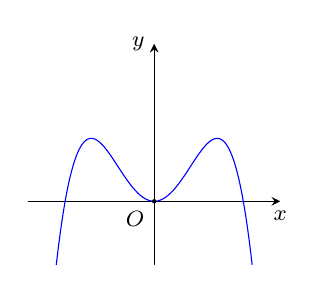
\begin{tikzpicture}[scale=0.8, font=\footnotesize,line join=round, line cap=round,>=stealth]
		\draw[->] (-2,0)--(0,0)node[below left]{$O$}--(2,0) node[below]{$x$};
		\draw[->] (0,-1)--(0,2.5) node [left]{$y$};
		\begin{scope}
			\clip (-2,-1) rectangle (2,2);
			\draw[blue,smooth,samples=100] plot[domain=-2:2](\x,{-(\x)^4+2*(\x)^2});
		\end{scope}
		\fill[black] (0,0) circle(1pt);
	\end{tikzpicture}
\end{center}
}
\end{ex}

\begin{ex}%[Đỗ Đường Hiếu, ĐMH-2023]%[2D1Y5-1]
\immini{Đường cong ở hình vẽ bên là đồ thị của hàm số nào dưới đây?
\choice
{$y=\dfrac{x-1}{x+1}$}
{$y=x^3-3x^2-1$}
{$y=-x^3+3x+1$}
{\True $y=\dfrac{x+1}{x-1}$}}
{\begin{tikzpicture}[scale=0.6, font=\footnotesize,line join=round, line cap=round,>=stealth]
			\draw[->] (-3,0)--(0,0)node[above left]{$O$}--(5,0) node[below]{$x$};
			\draw[->] (0,-3)--(0,5) node [left]{$y$};
				\begin{scope}
				\clip (-3,-3) rectangle (5,5);
				\draw[blue,smooth,samples=100] plot[domain=1.45:5](\x,{(\x+1)/(\x-1)}) plot[domain=-3:.55](\x,{(\x+1)/(\x-1)});
			\end{scope}
			\draw(1,5)--(1,-3) (-3,1)--(5,1);
			\fill[black] (0,0) circle(1pt);
	\end{tikzpicture}}
	\loigiai{
	Đồ thị hàm số đã cho có đường tiệm cận đứng $ x=x_0>0$ và đường tiệm cận ngang là $ y=y_0>0$.\\
	Nên trong các hàm số đã cho chỉ có đồ thị hàm số $y=\dfrac{x+1}{x-1}$ thỏa mãn.
	}
\end{ex}

\begin{ex}%[Đỗ Đường Hiếu, ĐMH-2023]%[2D1Y5-1]
\immini{Đồ thị sau đây là của hàm số nào?
\choice
{$y=-x^3+3x^2+1$}
{\True $y=x^3-3x+1$}
{$ y=-x^3-3x^2-1$}
{$ y=x^3-3x-1$}}
{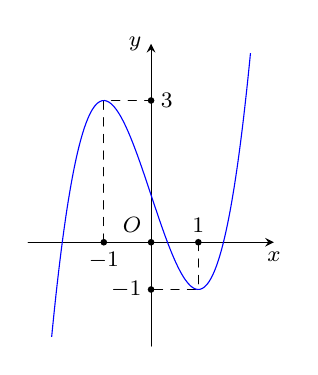
\begin{tikzpicture}[scale=0.6, font=\footnotesize,line join=round, line cap=round,>=stealth]
		\draw[->] (-2.6,0)--(0,0)node[above left]{$O$}--(2.6,0) node[below]{$x$};
		\draw[->] (0,-2.2)--(0,4.2) node [left]{$y$};
		\draw[dashed] (-1,0)|-(0,3);
		\draw[dashed] (1,0)|-(0,-1);
		\begin{scope}
			\clip (-2.5,-2) rectangle (2.5,4);
			\draw[blue,smooth,samples=100] plot[domain=-2.5:2.5](\x,{(\x)^3-3*(\x)+1});
		\end{scope}
		\fill[black] 
		(0,0) circle(2pt) 
		(-1,0)node[below]{$-1$} circle(2pt)
		(1,0)node[above]{$1$} circle(2pt)
		(0,-1)node[left]{$-1$} circle(2pt)
		(0,3)node[right]{$3$} circle(2pt);
\end{tikzpicture}}
\loigiai{
Hàm số có dạng $ y=ax^3+bx^2+cx+d$. Dựa vào đồ thị hàm số ta có
\begin{itemize}
	\item Hệ số $ a>0$.
	\item Đồ thị hàm số có hai điểm cực trị lần lượt là $A(-1;3)$ và $B(1;-1)$.
\end{itemize}
Trong các hàm số đã cho, chỉ có hàm số $y=x^3-3x+1$ thỏa mãn.
}
\end{ex}

\begin{ex}%[Đỗ Đường Hiếu, ĐMH-2023]%[2D1Y5-1]
\immini{Đường cong trong hình vẽ bên là đồ thị của hàm số nào dưới đây?
\choice 
{\True $y=x^3-3x-1$}
{$y=x^4-3x^2-1$}
{$y=-x^3-3x-1$}
{$y=-x^4+x^2-1$}}
{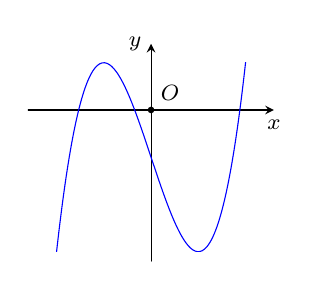
\begin{tikzpicture}[scale=0.6, font=\footnotesize,line join=round, line cap=round,>=stealth]
	\draw[->] (-2.6,0)--(0,0)node[above right]{$O$}--(2.6,0) node[below]{$x$};
	\draw[->] (0,-3.2)--(0,1.4) node [left]{$y$};
	\begin{scope}
		\clip (-2.5,-3) rectangle (2.5,1);
		\draw[blue,smooth,samples=100] plot[domain=-2.5:2.5](\x,{(\x)^3-3*(\x)-1});
	\end{scope}
	\fill[black] (0,0) circle (2pt);
\end{tikzpicture}}
\loigiai{
	Đồ thị hàm số là đồ thị của hàm số bậc ba có hệ số $a>0$.\\
 Nên chỉ có hàm số $y=x^3-3x-1$ thỏa mãn.
}
\end{ex}

\begin{ex}%[Đỗ Đường Hiếu, ĐMH-2023]%[2D1Y5-1]
	\immini{Đường cong trong hình vẽ bên là đồ thị của hàm số nào dưới đây?
		\choice 
		{$y=-x^3+3x^2$}
		{$y=x^4+2x^2$}
		{$y=x^3-3x^2$}
		{\True $y=-x^4+2x^2$}}
	{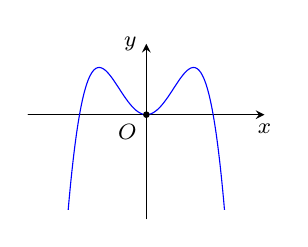
\begin{tikzpicture}[scale=0.6, font=\footnotesize,line join=round, line cap=round,>=stealth]
			\draw[->] (-2.5,0)--(0,0)node[below left]{$O$}--(2.5,0) node[below]{$x$};
			\draw[->] (0,-2.2)--(0,1.5) node [left]{$y$};
			\begin{scope}
				\clip (-2.5,-2) rectangle (2.5,1.5);
				\draw[blue,smooth,samples=100] plot[domain=-2:2](\x,{-(\x)^4+2*(\x)^2});
			\end{scope}
			\fill[black] (0,0) circle (2pt);
	\end{tikzpicture}}
	\loigiai{
		Đồ thị hàm số là đồ thị của hàm số dạng $y=ax^4+bx^2+c$ có hệ số $a<0$ nên chỉ có hàm số $y=-x^4+2x^2$ thỏa mãn.
	}
\end{ex}

\begin{ex}%[Đỗ Đường Hiếu, ĐMH-2023]%[2D1Y5-1]
	\immini{Đường cong trong hình vẽ bên là đồ thị của hàm số nào dưới đây?
		\choice 
		{$y=x^4-2x^2+1$}
		{$y=-x^4+2x^2+1$}
		{\True $y=-x^3+3x+1$}
		{$y=x^3-3x+1$}}
	{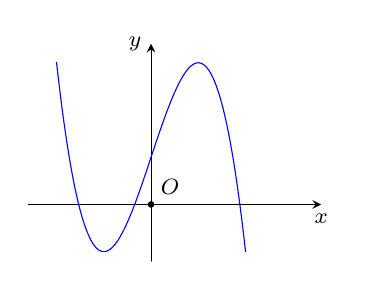
\begin{tikzpicture}[scale=0.6, font=\footnotesize,line join=round, line cap=round,>=stealth]
			\draw[->] (-2.6,0)--(0,0)node[above right]{$O$}--(3.6,0) node[below]{$x$};
			\draw[->] (0,-1.2)--(0,3.4) node [left]{$y$};
			\begin{scope}
				\clip (-2.5,-1) rectangle (3.5,3);
				\draw[blue,smooth,samples=100] plot[domain=-2.5:3.5](\x,{-(\x)^3+3*(\x)+1});
			\end{scope}
			\fill[black] (0,0) circle (2pt);
	\end{tikzpicture}}
	\loigiai{
		Đồ thị hàm số là đồ thị của hàm số bậc ba có hệ số $a<0$.\\
		Nên chỉ có hàm số $y=-x^3+3x+1$ thỏa mãn.
	}
\end{ex}

\begin{ex}%[Đỗ Đường Hiếu, ĐMH-2023]%[2D1Y5-1]
	\immini{Đường cong trong hình vẽ bên là đồ thị của hàm số nào dưới đây?
		\choice 
		{\True $y=x^4-2x^2+2$}
		{$y=x^3-x^2+2$}
		{$y=x^3-x+2$}
		{$y=-x^4+x^2+2$}}
	{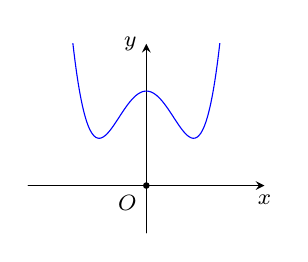
\begin{tikzpicture}[scale=0.6, font=\footnotesize,line join=round, line cap=round,>=stealth]
			\draw[->] (-2.5,0)--(0,0)node[below left]{$O$}--(2.5,0) node[below]{$x$};
			\draw[->] (0,-1)--(0,3) node [left]{$y$};
			\begin{scope}
				\clip (-2.5,-0.5) rectangle (2.5,3);
				\draw[blue,smooth,samples=100] plot[domain=-2:2](\x,{(\x)^4-2*(\x)^2+2});
			\end{scope}
			\fill[black] (0,0) circle (2pt);
	\end{tikzpicture}}
	\loigiai{
		Đồ thị hàm số là đồ thị của hàm số dạng $y=ax^4+bx^2+c$ có hệ số $a>0$.\\
		Nên chỉ có hàm số $y=x^4-2x^2+2$ thỏa mãn.
	}
\end{ex}

%Câu 9
\begin{ex}%[Đỗ Đường Hiếu, ĐMH-2023]%[2D1Y5-1]
	\immini{Đường cong ở hình vẽ bên là đồ thị của hàm số nào dưới đây?
		\choice
		{$y=\dfrac{x-2}{x+1}$}
		{$y=\dfrac{x+2}{x-1}$}
		{$y=\dfrac{x+2}{x-2}$}
		{\True $y=\dfrac{x-2}{x-1}$}}
	{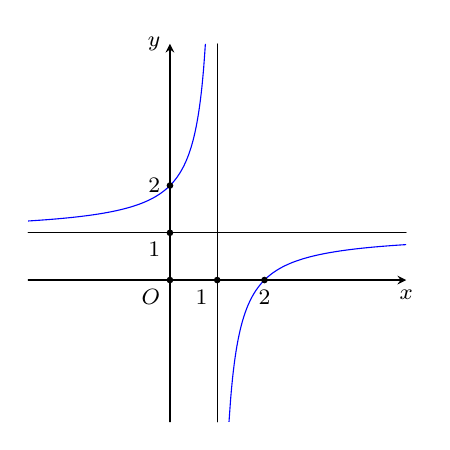
\begin{tikzpicture}[scale=0.6, font=\footnotesize,line join=round, line cap=round,>=stealth]
			\draw[->] (-3,0)--(0,0)node[below left]{$O$}--(5,0) node[below]{$x$};
			\draw[->] (0,-3)--(0,5) node [left]{$y$};
			\begin{scope}
				\clip (-3,-3) rectangle (5,5);
				\draw[blue,smooth,samples=100] plot[domain=1.25:5](\x,{(\x-2)/(\x-1)}) plot[domain=-3:.75](\x,{(\x-2)/(\x-1)});
			\end{scope}
			\draw(1,5)--(1,-3) (-3,1)--(5,1);
			\fill[black] 
			(0,0) circle(2pt) 
			(1,0) node[below left]{$1$} circle(2pt)
			(2,0) node[below]{$2$} circle(2pt)
			(0,1) node[below left]{$1$} circle(2pt)
			(0,2) node[left]{$2$} circle(2pt);
	\end{tikzpicture}}
	\loigiai{
		Đồ thị hàm số đã cho có đường tiệm cận đứng $x=1$ và đường tiệm cận ngang là $y=1$.\\
		Mặt khác đồ thị hàm số đi qua điểm $(0;2)$.\\
		Nên trong các hàm số đã cho chỉ có hàm số $y=\dfrac{x-2}{x-1}$ thỏa mãn.
	}
\end{ex}

%Câu 10
\begin{ex}%[Đỗ Đường Hiếu, ĐMH-2023]%[2D1Y5-1]
	\immini{Đường cong ở hình vẽ bên là đồ thị của hàm số nào dưới đây?
		\choice
		{$y=\dfrac{1-2x}{x+1}$}
		{$y=\dfrac{2x+1}{x+1}$}
		{$y=\dfrac{2x+1}{x-1}$}
		{\True $y=\dfrac{2x-1}{x+1}$}}
	{\begin{tikzpicture}[scale=0.6, font=\footnotesize,line join=round, line cap=round,>=stealth]
			\draw[->] (-4.5,0)--(0,0)node[above left]{$O$}--(3.5,0) node[below]{$x$};
			\draw[->] (0,-3)--(0,7) node [right]{$y$};
			\begin{scope}
				\clip (-4.5,-3) rectangle (3.5,7);
				\draw[blue,smooth,samples=100] plot[domain=-0.75:3.5](\x,{(2*(\x)-1)/(\x+1)}) plot[domain=-4.5:-1.25](\x,{(2*(\x)-1)/(\x+1)});
			\end{scope}
			\draw(-1,7)--(-1,-3) (-4.5,2)--(3.5,2);
			\fill[black] 
			(0,0) circle(2pt) 
			(-1,0) node[below left]{$-1$} circle(2pt)
			(0,-1) node[right]{$-1$} circle(2pt)
			(0,2) node[above right]{$2$} circle(2pt);
	\end{tikzpicture}}
	\loigiai{
		Hàm số có đồ thị trong đề bài có dạng $y=\dfrac{ax+b}{cx+d}$ với $c\ne 0$, $ad-bc\ne 0$.\\
		Dựa vào đồ thị ta có đường thẳng $x=-1$ là tiệm cận đứng, $y=2$ là tiệm cận ngang, đồ thị hàm số đi qua điểm $(0;-1)$. Trong các hàm số đã cho, chỉ có hàm số $y=\dfrac{2x-1}{x+1}$ là thỏa mãn. 
	}
\end{ex}

%Câu 11
\begin{ex}%[Đỗ Đường Hiếu, ĐMH-2023]%[2D1Y5-1]
	\immini{Đường cong ở hình vẽ bên là đồ thị của hàm số nào dưới đây?
		\choice
		{$y=\dfrac{x+2}{x+1}$}
		{$y=x^3-3x^2+1$}
		{\True $y=\dfrac{x-1}{x+1}$}
		{$y=-x^4+2x^2+1$}}
	{\begin{tikzpicture}[scale=0.6, font=\footnotesize,line join=round, line cap=round,>=stealth]
			\draw[->] (-5,0)--(0,0)node[below left]{$O$}--(3,0) node[below]{$x$};
			\draw[->] (0,-3)--(0,5) node [left]{$y$};
			\begin{scope}
				\clip (-5,-3) rectangle (3,5);
				\draw[blue,smooth,samples=100] plot[domain=-.75:3](\x,{(\x-1)/(\x+1)}) plot[domain=-5:-1.25](\x,{(\x-1)/(\x+1)});
			\end{scope}
			\draw(-1,5)--(-1,-3) (-5,1)--(3,1);
			\fill[black] (0,0) circle(2pt);
	\end{tikzpicture}}
	\loigiai{
	Nhìn vào đồ thị hàm số ta thấy đây là đồ thị hàm số $y=\dfrac{ax+b}{cx+d}$ với $c\ne 0$, $ad-bc\ne 0$.\\
	Cũng từ đồ thị hàm số suy ra hàm số đồng biến trên mỗi khoảng xác định của nó.\\ Trong các hàm số đã cho, chỉ có hàm số $y=\dfrac{x-1}{x+1}$ là thỏa mãn. 
	}
\end{ex}

%Câu 13
\begin{ex}%[Đỗ Đường Hiếu, ĐMH-2023]%[2D1Y5-1]
	\immini{Đồ thị của hàm số nào dưới đây có dạng đường cong như hình vẽ?
		\choice 
		{$y=x^3-2x^2-2$}
		{$y=x^3-3x^2+2$}
		{$y=-x^4+3x^2+2$}
		{\True $y=x^4-3x^2+2$}}
	{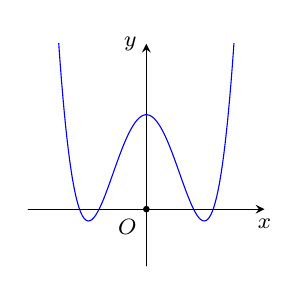
\begin{tikzpicture}[scale=0.6, font=\footnotesize,line join=round, line cap=round,>=stealth]
			\draw[->] (-2.5,0)--(0,0)node[below left]{$O$}--(2.5,0) node[below]{$x$};
			\draw[->] (0,-1.2)--(0,3.5) node [left]{$y$};
			\begin{scope}
				\clip (-2.5,-1) rectangle (2.5,3.5);
				\draw[blue,smooth,samples=100] plot[domain=-2:2](\x,{(\x)^4-3*(\x)^2+2});
			\end{scope}
			\fill[black] (0,0) circle (2pt);
	\end{tikzpicture}}
	\loigiai{
		Đồ thị hàm số là đồ thị của hàm số dạng $y=ax^4+bx^2+c$ có hệ số $a>0$.\\
		Nên chỉ có hàm số $y=x^4-3x^2+2$ thỏa mãn.
	}
\end{ex}

%Câu 15
\begin{ex}%[Đỗ Đường Hiếu, ĐMH-2023]%[2D1Y5-1]
	\immini{Đường cong ở hình vẽ bên là đồ thị của hàm số nào dưới đây?
		\choice
		{$y=\dfrac{x-1}{x+1}$}
		{$y=\dfrac{x+2}{x+1}$}
		{\True $y=\dfrac{2x+1}{x+1}$}
		{$y=\dfrac{x+3}{1-x}$}}
	{\begin{tikzpicture}[scale=0.6, font=\footnotesize,line join=round, line cap=round,>=stealth]
			\draw[->] (-4.5,0)--(0,0)node[below right]{$O$}--(3.5,0) node[below]{$x$};
			\draw[->] (0,-2)--(0,6) node [right]{$y$};
			\begin{scope}
				\clip (-4.5,-2) rectangle (3.5,6);
				\draw[blue,smooth,samples=100] plot[domain=-0.75:3.5](\x,{(2*(\x)+1)/(\x+1)}) plot[domain=-4.5:-1.25](\x,{(2*(\x)+1)/(\x+1)});
			\end{scope}
			\draw(-1,6)--(-1,-2) (-4.5,2)--(3.5,2);
			\fill[black] 
			(0,0) circle(2pt) 
			(-1,0) node[below left]{$-1$} circle(2pt)
			(0,1) node[right]{$1$} circle(2pt)
			(0,2) node[above right]{$2$} circle(2pt);
	\end{tikzpicture}}
	\loigiai{
		Dựa vào đồ thị ta có đường thẳng $x=-1$ là tiệm cận đứng, $y=2$ là tiệm cận ngang.\\ Trong các hàm số đã cho, chỉ có hàm số $y=\dfrac{2x+1}{x+1}$ là thỏa mãn. 
	}
\end{ex}

%Câu 18
\begin{ex}%[Đỗ Đường Hiếu, ĐMH-2023]%[2D1Y5-1]
	\immini{Đồ thị sau đây là của hàm số nào?
		\choice
		{$y=x^3+3x^2$}
		{$y=x^3+3x$}
		{\True $y=x^3-3x^2$}
		{$y=x^3-3x$}}
	{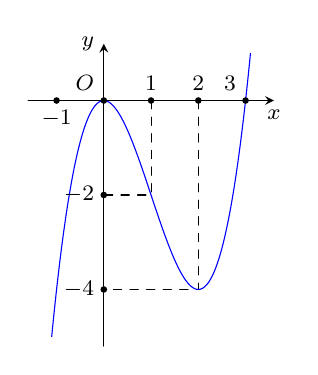
\begin{tikzpicture}[scale=0.6, font=\footnotesize,line join=round, line cap=round,>=stealth]
			\draw[->] (-1.6,0)--(0,0)node[above left]{$O$}--(3.6,0) node[below]{$x$};
			\draw[->] (0,-5.2)--(0,1.2) node [left]{$y$};
			\draw[dashed] (1,0)|-(0,-2);
			\draw[dashed] (2,0)|-(0,-4);
			\begin{scope}
				\clip (-1.5,-5) rectangle (3.5,1);
				\draw[blue,smooth,samples=100] plot[domain=-1.5:3.5](\x,{(\x)^3-3*(\x)^2});
			\end{scope}
			\fill[black] 
			(0,0) circle(2pt) 
			(-1,0)node[below]{$-1$} circle(2pt)
			(1,0)node[above]{$1$} circle(2pt)
			(2,0)node[above]{$2$} circle(2pt)
			(3,0)node[above left]{$3$} circle(2pt)
			(0,-2)node[left]{$-2$} circle(2pt)
			(0,-4)node[left]{$-4$} circle(2pt);
	\end{tikzpicture}}
	\loigiai{
	Ta có
	\begin{itemize}
		\item Đồ thị hàm số đi qua điểm có tọa độ $(1;-2)$ nên loại $y=x^3+3x^2$ và $y=x^3+3x$.
		\item Đồ thị hàm số đi qua điểm có tọa độ $(2;-4)$ nên loại $y=x^3-3x$.
	\end{itemize}
		Vậy chỉ có hàm số $y=x^3-3x^2$ thỏa mãn.
	}
\end{ex}

%Câu 19
\begin{ex}%[Đỗ Đường Hiếu, ĐMH-2023]%[2D1Y5-1]
	\immini{Đường cong ở hình vẽ bên là đồ thị của hàm số nào dưới đây?
		\choice
		{\True $y=\dfrac{x+1}{x-1}$}
		{$y=x^4+x^2+1$}
		{$y=x^3-3x-1$}
		{$y=\dfrac{2x-1}{x-1}$}}
	{\begin{tikzpicture}[scale=0.6, font=\footnotesize,line join=round, line cap=round,>=stealth]
			\draw[->] (-3,0)--(0,0)node[above left]{$O$}--(5,0) node[below]{$x$};
			\draw[->] (0,-3)--(0,5) node [left]{$y$};
			\begin{scope}
				\clip (-3,-3) rectangle (5,5);
				\draw[blue,smooth,samples=100] plot[domain=1.45:5](\x,{(\x+1)/(\x-1)}) plot[domain=-3:.55](\x,{(\x+1)/(\x-1)});
			\end{scope}
			\draw(1,5)--(1,-3) (-3,1)--(5,1);
			\fill[black] (0,0) circle(1pt);
	\end{tikzpicture}}
	\loigiai{
		Đồ thị hàm số đã cho có đường tiệm cận đứng $x=x_0>0$ và đường tiệm cận ngang là $y=y_0>0$, cắt trục tung tại điểm có tung độ $y=y_1<0$, nên trong các hàm số đã cho chỉ có hàm số $y=\dfrac{x+1}{x-1}$ thỏa mãn.
	}
\end{ex}

%Câu 24
\begin{ex}%[Đỗ Đường Hiếu, ĐMH-2023]%[2D1Y5-1]
	\immini{Đường cong trong hình vẽ bên là đồ thị của hàm số nào dưới đây?
		\choice 
		{$y=-x^3+3x+1$}
		{$y=x^4-3x^2+1$}
		{\True $y=x^3-3x+1$}
		{$y=x^2-3x+1$}}
	{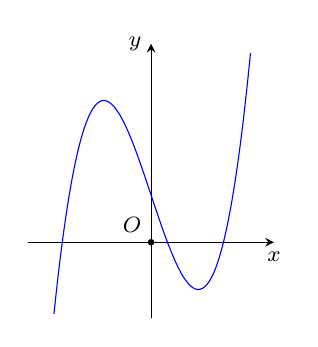
\begin{tikzpicture}[scale=0.6, font=\footnotesize,line join=round, line cap=round,>=stealth]
			\draw[->] (-2.6,0)--(0,0)node[above left]{$O$}--(2.6,0) node[below]{$x$};
			\draw[->] (0,-1.6)--(0,4.2) node [left]{$y$};
			\begin{scope}
				\clip (-2.5,-1.5) rectangle (2.5,4);
				\draw[blue,smooth,samples=100] plot[domain=-2.5:2.5](\x,{(\x)^3-3*(\x)+1});
			\end{scope}
			\fill[black] (0,0) circle (2pt);
	\end{tikzpicture}}
	\loigiai{
		Đồ thị hàm số là đồ thị của hàm số bậc ba có hệ số $a>0$.\\
		Nên chỉ có hàm số $y=x^3-3x+1$ thỏa mãn.
	}
\end{ex}

\begin{ex}%[Đỗ Đường Hiếu, ĐMH-2023]%[2D1Y5-1]
	\immini{
		Hình vẽ bên là đồ thị của hàm số nào?
		\choice
		{$y=x^3-3x+1$}
		{$y=x^4-2x^2+3$}
		{\True $y=x^3-3x^2+3x+1$}
		{$y=-x^3-3x^2-1$}
	}{
		\begin{tikzpicture}[scale=0.6, font=\footnotesize,line join=round, line cap=round,>=stealth]
			\draw[->] (-1.5,0) -- (0,0) node[below right]{$O$} -- (1,0) node[below]{$1$} -- (3.3,0) node[below]{$x$};
			\draw[->] (0,-1) -- (0,1) node[left]{$1$} -- (0,2) node[left]{$2$} -- (0,3.6) node[left]{$y$};
			\begin{scope}
				\clip (-1,-1) rectangle (3.5,3.5);
				\draw[blue,smooth,samples=100] plot[domain=-3:3](\x, {(\x)^3-3*(\x)^2+3*(\x)+1});
			\end{scope}
			\draw[dashed] (1,0) |- (0,2);
		\end{tikzpicture}
	}
	\loigiai{
		Vì đồ thị hàm số đi qua các điểm $(0;1)$ và $(1;2)$.\\
		Nên chỉ có hàm số $y=x^3-3x^2+3x+1$ thỏa mãn.
	}
\end{ex}


%Câu 21
\begin{ex}%[Đỗ Đường Hiếu, ĐMH-2023]%[2D1Y5-1]
Hàm số nào sau đây có bảng biến thiên như hình dưới?
\begin{center}
	
\begin{tikzpicture}
		\tkzTabInit[nocadre=false,lgt=1.3,espcl=2.5,deltacl=0.6]
		{$x$ /0.6,$f'(x)$ /0.6, $f(x)$ /2}
		{$-\infty$,$-1$,$1$,$+\infty$} 
		\tkzTabLine {,+,0,-,0,+,} 
		\tkzTabVar{-/ $-\infty $ , +/ $2$,-/$-2$,+/$+\infty $}  
	\end{tikzpicture}
\end{center}
\choice
{$y=-x^3+3x^2+1$}
{$y=-x^3+3x$}
{$y=x^3-3x^2-1$}
{\True $y=x^3-3x$}	
\loigiai{
Ta có $\lim\limits_{x\to +\infty}y=+\infty$ nên loại hai hàm số $y=-x^3+3x^2+1$ và $y=-x^3+3x$.\\
Phương trình $y'=0$ có hai nghiệm $x=\pm 1$.\\
Hàm số $y=x^3-3x$ có $y'=3x^2-3=0\Rightarrow x=\pm 1$.\\ Do đó hàm số $y=x^3-3x$ thỏa mãn.
}
\end{ex}


%Câu 22
\begin{ex}%[Đỗ Đường Hiếu, ĐMH-2023]%[2D1Y5-1]
	Hàm số nào sau đây có bảng biến thiên như hình dưới?
	\begin{center}
		
\begin{tikzpicture}
			\tkzTabInit[nocadre=false,lgt=1.3,espcl=2.5,deltacl=0.6]
			{$x$ /0.6,$f'(x)$ /0.6, $f(x)$ /2}
			{$-\infty$,$-1$,$1$,$+\infty$} 
			\tkzTabLine {,-,0,+,0,-,} 
			\tkzTabVar{+/ $+\infty $ , -/ $0$,+/$4$,-/$-\infty $}  
		\end{tikzpicture}
	\end{center}
	\choice
	{$y=x^4-2x^2-3$}
	{\True $y=-x^3+3x+2$}
	{$y=x^3-3x+4$}
	{$y=\dfrac{x-1}{2x-1}$}	
	\loigiai{
		Bảng biến thiên của hàm số bậc ba có hệ số $a<0$.\\
		Nên chỉ có hàm số $y=-x^3+3x+2$ thỏa mãn.
	}
\end{ex}


%Câu 23
\begin{ex}%[Đỗ Đường Hiếu, ĐMH-2023]%[2D1Y5-1]
	Hàm số nào sau đây có bảng biến thiên như hình dưới?
	\begin{center}
		
\begin{tikzpicture}
			\tkzTabInit[nocadre=false,lgt=1.3,espcl=2.5,deltacl=0.6]
			{$x$ /0.6,$f'(x)$ /0.6, $f(x)$ /2}
			{$-\infty$,$-1$,$0$,$1$,$+\infty$} 
			\tkzTabLine {,-,0,+,0,-,0,+,} 
			\tkzTabVar{+/ $+\infty $ , -/ $-4$,+/$-3$,-/$-4$,+/$-\infty $}  
		\end{tikzpicture}
	\end{center}
	\choice
	{\True $y=2|x^3|-3x^2-3$}
	{$y=2x^4-4x^2-3$}
	{$y=2|x^3|-3|x|-3$}
	{$y=\dfrac{1}{2}x^4-x^2-3$}	
	\loigiai{
		Từ bảng biến thiên ta có
		\begin{itemize}
			\item $y(\pm 1)=-4$ nên loại $y=2x^4-4x^2-3$ và $y=\dfrac{1}{2}x^4-x^2-3$.
			\item Hàm số $y=2|x^3|-3|x|-3$ không có đạo hàm tại $x=0$ nên hàm số $y=2|x^3|-3|x|-3$ không thỏa mãn.
		\end{itemize}
	Vậy hàm số $y=2|x^3|-3x^2-3$ thỏa mãn.
	}
\end{ex}


%Câu 25
\begin{ex}%[Đỗ Đường Hiếu, ĐMH-2023]%[2D1Y5-1]
	Hàm số nào sau đây có bảng biến thiên như hình dưới?
	\begin{center}
		
\begin{tikzpicture}
			\tkzTabInit[nocadre=false,lgt=1.3,espcl=2.5,deltacl=0.6]
			{$x$ /0.6,$f'(x)$ /0.6, $f(x)$ /2}
			{$-\infty$,$-1$,$+\infty$} 
			\tkzTabLine {,-,d,-,} 
			\tkzTabVar{+/$-2$, -D+/$-\infty $/$-\infty $,-/$-2$}  
		\end{tikzpicture}
	\end{center}
	\choice
	{\True $y=\dfrac{-2x+3}{x+1}$}
	{$y=\dfrac{-2x-4}{x+1}$}
	{$y=\dfrac{x-4}{2x+2}$}
	{$y=\dfrac{2-x}{x+1}$}	
	\loigiai{
		Dựa vào bảng biến thiên ta có tiệm cận đứng của đồ thị hàm số là đường thẳng $x=-1$; tiệm cận ngang là đường thẳng $y=-2$.\\
		Ta cũng có $y'<0,\forall x\ne -1$.\\
		Trong các hàm số đã cho, chỉ có hàm số $y=\dfrac{-2x+3}{x+1}$ thỏa mãn.
	}
\end{ex}




\Closesolutionfile{ans}
%======================
\subsection{Bảng đáp án}
\inputansbox{8}{ans/ANS-DANG-9}

